% ============================================================
%  SCHOLA DOMESTICA — Magister Mathematica
%  Level 1 | Week 10 | Day 2
%  Topic: Doubles Facts — 1+1 through 4+4
% ============================================================
\documentclass[12pt, letterpaper]{article}

\usepackage[top=1in, bottom=1in, left=1in, right=1in]{geometry}
\usepackage[T1]{fontenc}
\usepackage[utf8]{inputenc}
\usepackage{lmodern}
\usepackage{microtype}
\usepackage{amsmath}
\usepackage{xcolor}
\usepackage{tikz}
\usepackage{array}
\usepackage{enumitem}
\usepackage{multicol}
\usepackage{mdframed}
\usepackage{fancyhdr}

\definecolor{scholared}{RGB}{160,30,30}
\definecolor{scholagold}{RGB}{180,140,40}
\definecolor{scholacream}{RGB}{253,248,235}
\definecolor{scholagreen}{RGB}{50,110,60}
\definecolor{scholablue}{RGB}{40,80,140}

\pagestyle{fancy}
\fancyhf{}
\renewcommand{\headrulewidth}{0.6pt}
\fancyhead[L]{\small\textcolor{scholared}{\textbf{Schola Domestica — Magister Mathematica}}}
\fancyhead[R]{\small\textcolor{scholared}{Level 1 · Week 10 · Day 2}}
\fancyfoot[C]{\small\textcolor{gray}{— \thepage\ —}}

\newcommand{\answerline}{\underline{\hspace{2.5cm}}}
\newcommand{\biganswerline}{\underline{\hspace{4cm}}}
\newcommand{\numbox}{\tikz{\draw[scholablue,thick](0,0)rectangle(1.2cm,0.85cm);}}

\newmdenv[
  backgroundcolor=scholacream,
  linecolor=scholared,
  linewidth=1.5pt,
  roundcorner=6pt,
  innertopmargin=8pt,
  innerbottommargin=8pt,
  innerleftmargin=10pt,
  innerrightmargin=10pt
]{lessonbox}

\newmdenv[
  backgroundcolor={rgb,255:red,235;green,245;blue,235},
  linecolor=scholagreen,
  linewidth=1.2pt,
  roundcorner=4pt,
  innertopmargin=6pt,
  innerbottommargin=6pt,
  innerleftmargin=8pt,
  innerrightmargin=8pt
]{enrichbox}

\begin{document}

\begin{center}
  {\LARGE\textbf{\textcolor{scholared}{Doubles!}}}\\[4pt]
  {\Large\textcolor{scholagold}{\textit{When Both Parts Are the Same}}}\\[6pt]
  {\small Name: \biganswerline \hspace{1cm} Date: \answerline}
\end{center}

\vspace{4pt}
\noindent\textcolor{scholared}{\rule{\linewidth}{1pt}}
\vspace{4pt}

% IMAGE PROMPT (Miyazaki watercolour style):
% Two identical small tanuki (raccoon dogs) face each other on a mossy stone, each holding exactly
% three red berries. Mirror-image composition, soft forest morning light, green and amber palette,
% white paper background, no text.

\begin{lessonbox}
\textbf{A doubles fact} has the \emph{same number} added to itself.\\[6pt]
\noindent
\begin{tabular}{@{}p{3.5cm} p{3.5cm} p{3.5cm}@{}}
$1 + 1 = \mathbf{2}$ & $2 + 2 = \mathbf{4}$ & $3 + 3 = \mathbf{6}$ \\[4pt]
\textit{mirror hands} & \textit{two eyes, two ears} & \textit{two triangles}
\end{tabular}

\medskip
\noindent\textbf{Memory trick:} Doubles always give an \emph{even} answer: 2, 4, 6, 8, 10\ldots
\end{lessonbox}

\bigskip

% ===== PART I: DOUBLES PICTURES =====
\noindent\textcolor{scholared}{\large\textbf{Part I — Doubles with Pictures}} \hfill \textit{(Problems 1–5)}

\medskip
\noindent\textit{Both groups are the same. Count all. Write the doubles fact.}

\bigskip

% Row of doubles diagrams
\noindent
\begin{tabular}{@{}p{2.8cm} p{2.8cm} p{2.8cm} p{2.8cm} p{2.8cm}@{}}

% 1: 1+1=2
\textbf{1.}\quad
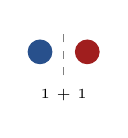
\begin{tikzpicture}[baseline=0]
  \filldraw[scholablue] (0,0.3) circle (0.15cm);
  \draw[dashed,gray] (0.3,0) -- (0.3,0.6);
  \filldraw[scholared] (0.6,0.3) circle (0.15cm);
  \node[below] at (0.3,-0.05) {\tiny 1 + 1};
\end{tikzpicture}\\
$1 + 1 =$ \numbox
&
% 2: 2+2=4
\textbf{2.}\quad
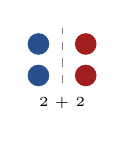
\begin{tikzpicture}[baseline=0]
  \foreach \y in {0.1,0.5} { \filldraw[scholablue] (0,\y) circle (0.13cm); }
  \draw[dashed,gray] (0.3,0) -- (0.3,0.7);
  \foreach \y in {0.1,0.5} { \filldraw[scholared] (0.6,\y) circle (0.13cm); }
  \node[below] at (0.3,-0.05) {\tiny 2 + 2};
\end{tikzpicture}\\
$2 + 2 =$ \numbox
&
% 3: 3+3=6
\textbf{3.}\quad
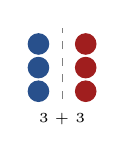
\begin{tikzpicture}[baseline=0]
  \foreach \y in {0,0.3,0.6} { \filldraw[scholablue] (0,\y) circle (0.13cm); }
  \draw[dashed,gray] (0.3,-0.1) -- (0.3,0.8);
  \foreach \y in {0,0.3,0.6} { \filldraw[scholared] (0.6,\y) circle (0.13cm); }
  \node[below] at (0.3,-0.15) {\tiny 3 + 3};
\end{tikzpicture}\\
$3 + 3 =$ \numbox
&
% 4: 4+4=8
\textbf{4.}\quad
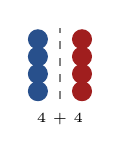
\begin{tikzpicture}[baseline=0]
  \foreach \y in {0,0.22,0.44,0.66} { \filldraw[scholablue] (0,\y) circle (0.12cm); }
  \draw[dashed,gray] (0.28,-0.1) -- (0.28,0.8);
  \foreach \y in {0,0.22,0.44,0.66} { \filldraw[scholared] (0.56,\y) circle (0.12cm); }
  \node[below] at (0.28,-0.15) {\tiny 4 + 4};
\end{tikzpicture}\\
$4 + 4 =$ \numbox
&
% 5: 0+0=0
\textbf{5.}\\[6pt]
$0 + 0 =$ \numbox\\
\textit{\small (nothing + nothing)}

\end{tabular}

\bigskip\bigskip

% ===== PART II: DOUBLES MIXED =====
\noindent\textcolor{scholared}{\large\textbf{Part II — Solve and Colour}} \hfill \textit{(Problems 6–10)}

\medskip
\noindent\textit{Solve each doubles fact. If the answer is \textbf{even}, colour the box gold.}

\bigskip

\noindent
\begin{tabular}{@{}p{3.0cm} p{3.0cm} p{3.0cm} p{3.0cm}@{}}
\textbf{6.}\; $2 + 2 =$ \numbox &
\textbf{7.}\; $4 + 4 =$ \numbox &
\textbf{8.}\; $3 + 3 =$ \numbox &
\textbf{9.}\; $1 + 1 =$ \numbox
\end{tabular}

\medskip

\noindent\textbf{10.} Write the missing double: \quad $\numbox + \numbox = 6$

\bigskip\bigskip

% ===== PART III: MIXED +4, +5, DOUBLES =====
\noindent\textcolor{scholared}{\large\textbf{Part III — Mixed Facts: $+4$, $+5$, Doubles}} \hfill \textit{(Problems 11–16)}

\bigskip

\noindent
\begin{tabular}{@{}p{3.3cm} p{3.3cm} p{3.3cm} p{3.3cm}@{}}
\textbf{11.}\; $4 + 3 =$ \numbox &
\textbf{12.}\; $3 + 5 =$ \numbox &
\textbf{13.}\; $2 + 4 =$ \numbox &
\textbf{14.}\; $4 + 4 =$ \numbox \\[12pt]
\multicolumn{2}{@{}l@{}}{\textbf{15.}\; $5 + 2 =$ \numbox} &
\multicolumn{2}{@{}l@{}}{\textbf{16.}\; $4 + 1 =$ \numbox}
\end{tabular}

\bigskip

\begin{enrichbox}
\textbf{\textcolor{scholagreen}{Doubles Song (say aloud to any tune!):}}\\[4pt]
\textit{``1 plus 1 is 2, \quad 2 plus 2 is 4,}\\
\textit{3 plus 3 is 6, \quad and 4 plus 4 is more —}\\
\textit{4 plus 4 is 8!''}\\[4pt]
\noindent Repeat 3 times until it is remembered by heart.
\end{enrichbox}

\vspace{0.3cm}
\noindent\textcolor{gray}{\small\textit{Ray's Primary Arithmetic — doubles and counting on.}}

\end{document}
